\documentclass{article}

\usepackage[margin=1.0in]{geometry}
\usepackage{upgreek}
\usepackage{amsmath}
\usepackage{minted}
\usepackage{graphicx}
\usepackage{caption}
\usepackage{subcaption}
\usepackage{mathrsfs}
\usepackage[toc,page]{appendix}

%Section style
\usepackage{etoolbox} %for configuration of sloppy
\usepackage{xcolor}


\definecolor{secnum}{RGB}{102,102,102}

\makeatletter
    \def\@seccntformat#1{\llap{\color{secnum}\csname the#1\endcsname\hskip 16pt}}
\makeatother
%end section style

\begin{document}

\begin{titlepage}
\begin{center}
    \hline \\[0.2cm]
\textsc{\Large Statistical methods for machine learning}\\[0.5cm]
\textsc{\large Assignment 2}\\[0.5cm]
    \hline
    \hline
\vspace{2 cm}
\begin{tabular}{ll}
Students: & Lasse Ahlbech Madsen \\
          & Kasper Passov\\
\end{tabular}
\end{center}
\vspace{5 cm}
% \tableofcontents
\newpage
\end{titlepage}

\section{III.1}

\subsection{Deriviation of the derivative of the transfer function}
\subsection{proof}

For the hidden neurons, we have the non-linearity (transfer function, activation function)
\begin{equation*}
    h(a) = \frac{a}{1 + |a|}
\end{equation*}
And we wish to find its derivitive 

\begin{equation*}
    h'(a) = \frac{d}{da}\frac{a}{1 + |a|}
\end{equation*}
We start by using the quotient rule 

\begin{equation*}
    \frac{d}{da} \frac{u}{v} = \frac{v \frac{du}{dv} - u\frac{dv}{du}}{v^2}
\end{equation*}
Where $u = a$ and $v = |a| + 1$

\begin{equation*}
    \frac{(1 + |a|) (\frac{d}{da}(a)) - a(\frac{d}{da}(1 + |a|))}{(1 + |a|)^2}
\end{equation*}
The derivative of a is 1

\begin{equation*}
    \frac{(1 + |a|)(1) - a(\frac{d}{da}(1 + |a|))}{(1 + |a|)^2}
\end{equation*}
Simplify:

\begin{equation*}
    \frac{1 + |a| - a(\frac{d}{da}(1 + |a|))}{(1 + |a|)^2}
\end{equation*}
We split up the term and differentiate independently:

\begin{equation*}
    \frac{1 + |a| - a(\frac{d}{da}(1) + \frac{d}{da}(|a|))}{(1 + |a|)^2}
\end{equation*}
the derivation of 1 is 0

\begin{equation*}
    \frac{1 + |a| - a(\frac{d}{da}(|a|))}{(1 + |a|)^2}
\end{equation*}
the derivation of $|a|$ is $\frac{a}{|a|}$

\begin{equation*}
    \frac{1 + |a| - a(\frac{a}{|a|})}{(1 + |a|)^2}
\end{equation*}
Simplify:

\begin{equation} \label{mathlol}
    \frac{1 + |a| - \frac{a^2}{|a|}}{(1 + |a|)^2}
\end{equation}
If $a = 0$ we try (\ref{mathlol}):

\begin{equation*}
    \frac{1 + 0 - \frac{0^2}{0}}{(1 + 0)^2}\\
\end{equation*}
This becomes impossible as we try to divide by zero.\\
With both $a > 0$ and $a < 0$ means $|a| = a$ we use (\ref{mathlol}):
\begin{equation*}
    &\frac{1 + a - \frac{a^2}{a}}{(1 + a)^2}\\
\end{equation*}
Simplify:

\begin{equation*}
    h'(a) = \frac{1}{(1 + |a|)^2}
\end{equation*}

\subsection{}


\begin{figure}
    \centering
    \begin{subfigure}[b]{0.49\textwidth}
        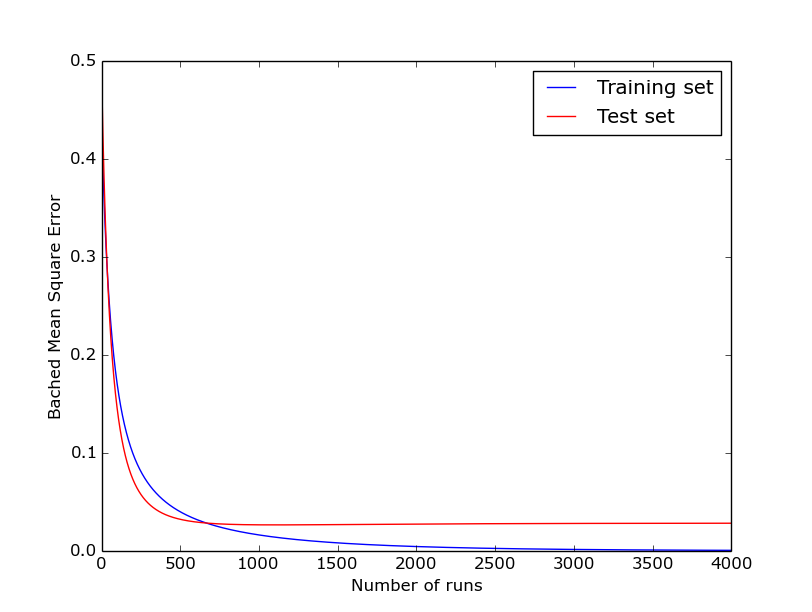
\includegraphics[width=1.0\textwidth]{Part1/20Nodes.png}
        \caption{20 Nodes}
        \label{fig:2scatter}
    \end{subfigure}
    \begin{subfigure}[b]{0.49\textwidth}
        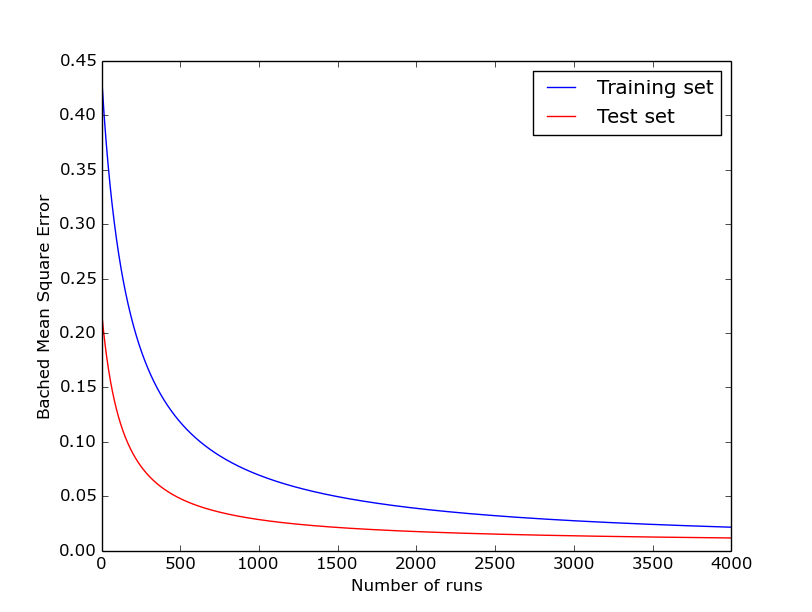
\includegraphics[width=1.0\textwidth]{Part1/2Nodes.png}
        \caption{2 Nodes} 
        \label{fig:2scatter}
    \end{subfigure}
    \caption{Error calculation as a function of runs with learning and momentum constants set to 0.05}
    \label{}
\end{figure}

\section{III.2}

The code for this section can be found in Part2/. The script
"Opgaveiii21.m executes the entire thing.

\subsection{III.2.1}

\iffalse
  HAHAHAHAHAHHAHAHAHAHAHAHAHAHAHAHAHAHHAHA nej
\begin{table}[h!]
  \begin{tabular}{l|l|l|l|l|l|l|l|l|l|l|l|l|l|l|l|l|l|l|l|l|l|l}
    & Attribute 1 & Attribute 2 & Attribute 3 & Attribute 4 & Attribute 5 &
    Attribute 6 & Attribute 7 & Attribute 8 & Attribute 9 & Attribute 10 &
    Attribute 11 & Attribute 12 & Attribute 13 & Attribute 14 & Attribute
    15 & Attribute 16 & Attribute 17 & Attribute 18 & Attribute 19 &
    Attribute 20 & Attribute 21 & Attribute 22 \\
    Mean traindata & 155.9604 & 204.8212 & 115.0586  &  0.0060 &   0.0000 &   
    0.0032 & 0.0033 &   0.0096 &   0.0277 &   0.2624 &   0.0147 &   0.0166 & 
    0.0220 &  0.0440  &  0.0226  & 22.0007  &  0.4948 &   0.7157 &  -5.7637 &
    0.2148&    2.3658 &   0.1997 \\
    Variance traindata & 1.9830  &  9.7331 &   2.1152  &  0.0000 &
    0.0000 &  0.0000  &  0.0000 &   0.0000 &   0.0000  &  0.0000  &
    0.0000 &   0.0000 &  0.0000 &   0.0000    & 0.0000 &   0.0167  &
    0.0000 & 0.0000  &  0.0011  &  0.0000 &   0.0001 &   0.0000 \\
    Mean normalized testdata &  -0.0782 &  -0.1572  &  0.0553 &   0.1126 &
    0.0712 &   0.0865  &  0.1151 &   0.0866  &  0.2477  &  0.2439 &
    0.2284 &   0.2496 & 0.3150 &   0.2284 &   0.1483 &  -0.0565 &   0.0732
    &    0.0863 &   0.1540 &   0.3091 &   0.0870  &  0.1677 
    
  \end{tabular}
  \label{tab:meanvar}
  \caption{The mean and variance of the data. First the unnormalized traindata,
  then the normalized testdata.}
\end{table}
\end{comment}

\fi

Below is a printout of the mean and variance of the untransformed
traindata attribute and the transformed testdata attributes. The
testdata obviously does not have zero mean and unit variance as it is
transformed with the mean and standard deviation of the traindata.

\begin{minted}{matlab}
>> mean(traindata)

ans =

  Columns 1 through 12

  155.9604  204.8212  115.0586    0.0060    0.0000    0.0032    0.0033    0.0096    0.0277    0.2624    0.0147    0.0166

  Columns 13 through 22

    0.0220    0.0440    0.0226   22.0007    0.4948    0.7157   -5.7637    0.2148    2.3658    0.1997

>> var(traindata)

ans =

   1.0e+03 *

  Columns 1 through 12

    1.9830    9.7331    2.1152    0.0000    0.0000    0.0000    0.0000    0.0000    0.0000    0.0000    0.0000    0.0000

  Columns 13 through 22

    0.0000    0.0000    0.0000    0.0167    0.0000    0.0000    0.0011    0.0000    0.0001    0.0000

>> mean(normtest)

ans =

  Columns 1 through 12

   -0.0782   -0.1572    0.0553    0.1126    0.0712    0.0865    0.1151    0.0866    0.2477    0.2439    0.2284    0.2496

  Columns 13 through 22

    0.3150    0.2284    0.1483   -0.0565    0.0732    0.0863    0.1540    0.3091    0.0870    0.1677

>> var(normtest)

ans =

  Columns 1 through 12

    0.7323    0.7150    0.7977    1.9906    1.6662    2.1370    1.9225    2.1379    1.7721    1.8292    1.7175    1.7780

  Columns 13 through 22

    2.1905    1.7176    2.6633    1.3610    1.0827    0.9514    1.2166    1.3629    1.1336    1.4149
\end{minted}

\subsection{III.2.2}

We used LIBSVM to train our model. It makes it possible to specify a
kernel function of your liking and choose a $\gamma$ and a $C$ of your
choosing, so we did not look further.

We did the crossvalidation by splitting the data into 5 parts. Three of
size 20 and two of size 19. Additionally we for both the raw and the
normalised data made a list of size 7 for possible $\gamma$'s and the
same for C. We it for both since the two datasets are of very different
sizes. Then we trained a model for each combination and chose the one
with the lowest 0-1 loss and used the found values to train the new model.

On the unnormalized data we observed a 0-1 loss of 18.56 \% on the trainingdata
and 21.43 \% on the testdata. OUr gridsearch resulted in a C of 100 and
a $\gamma$  of $2^{-20}$. 

On the normalized data the 0-1 loss on the trainingdata was 10.20 \%
and 13.40 \% on the testdata. The best C was 100 and the best
$\gamma$ was $2^{-10}$.

Without normalization some features weigh much more than others and the
model ends up practically ignoring the rest of the colums. Particularly
the first three columns are quite a bit higher than the other columns.

\subsection{III.2.3}
For the following section we will use the normalized data.

\subsubsection{III.2.3.1}
In our model there are 31 bounded support vectors and 10 free support
vectors. 

Decreasing C increases the number of support vectors and all of
them will eventually become bounded vectors. This could result in
underfitting and will increase the number of training errors.

Drastically increasing C will lower the amount of support vectors which
will cause the model to overfit and outliers will distort the hyperplane
to a greater degree.


\subsection{III.2.3.2}

More data will result in more support vectors. This will give increased
precision, but also a potential cost in performance of the model. For
large scale application it may be a good idea to increase C to lower the
amount of support vectors to hasten the computations.

\end{document}
